%%%%%%%%%%%%%%%%%%%%%%%%%%%%%%%%%%%%%%%%%
% Programming/Coding Assignment
% LaTeX Template
%
% This template has been downloaded from:
% http://www.latextemplates.com
%
% Original author:
% Ted Pavlic (http://www.tedpavlic.com)
%
% Note:
% The \lipsum[#] commands throughout this template generate dummy text
% to fill the template out. These commands should all be removed when 
% writing assignment content.
%
% This template uses a Perl script as an example snippet of code, most other
% languages are also usable. Configure them in the "CODE INCLUSION 
% CONFIGURATION" section.
%
%%%%%%%%%%%%%%%%%%%%%%%%%%%%%%%%%%%%%%%%%

%----------------------------------------------------------------------------------------
%	PACKAGES AND OTHER DOCUMENT CONFIGURATIONS
%----------------------------------------------------------------------------------------

\documentclass{article}

\usepackage{fancyhdr} % Required for custom headers
\usepackage{lastpage} % Required to determine the last page for the footer
\usepackage{extramarks} % Required for headers and footers
\usepackage[usenames,dvipsnames]{color} % Required for custom colors
\usepackage{graphicx} % Required to insert images
\usepackage{subcaption}
\usepackage{listings} % Required for insertion of code
\usepackage{courier} % Required for the courier font
\usepackage{lipsum} % Used for inserting dummy 'Lorem ipsum' text into the template

% Margins
\topmargin=-0.45in
\evensidemargin=0in
\oddsidemargin=0in
\textwidth=6.5in
\textheight=9.0in
\headsep=0.25in

\linespread{1.1} % Line spacing

% Set up the header and footer
\pagestyle{fancy}
\lhead{\hmwkAuthorName} % Top left header
\chead{\hmwkClass\ (\hmwkClassTime): \hmwkTitle} % Top center head
%\rhead{\firstxmark} % Top right header
\lfoot{\lastxmark} % Bottom left footer
\cfoot{} % Bottom center footer
\rfoot{Page\ \thepage\ of\ \protect\pageref{LastPage}} % Bottom right footer
\renewcommand\headrulewidth{0.4pt} % Size of the header rule
\renewcommand\footrulewidth{0.4pt} % Size of the footer rule

\setlength\parindent{0pt} % Removes all indentation from paragraphs

%----------------------------------------------------------------------------------------
%	CODE INCLUSION CONFIGURATION
%----------------------------------------------------------------------------------------

\definecolor{MyDarkGreen}{rgb}{0.0,0.4,0.0} % This is the color used for comments
\lstloadlanguages{Perl} % Load Perl syntax for listings, for a list of other languages supported see: ftp://ftp.tex.ac.uk/tex-archive/macros/latex/contrib/listings/listings.pdf
\lstset{language=Perl, % Use Perl in this example
        frame=single, % Single frame around code
        basicstyle=\small\ttfamily, % Use small true type font
        keywordstyle=[1]\color{Blue}\bf, % Perl functions bold and blue
        keywordstyle=[2]\color{Purple}, % Perl function arguments purple
        keywordstyle=[3]\color{Blue}\underbar, % Custom functions underlined and blue
        identifierstyle=, % Nothing special about identifiers                                         
        commentstyle=\usefont{T1}{pcr}{m}{sl}\color{MyDarkGreen}\small, % Comments small dark green courier font
        stringstyle=\color{Purple}, % Strings are purple
        showstringspaces=false, % Don't put marks in string spaces
        tabsize=5, % 5 spaces per tab
        %
        % Put standard Perl functions not included in the default language here
        morekeywords={rand},
        %
        % Put Perl function parameters here
        morekeywords=[2]{on, off, interp},
        %
        % Put user defined functions here
        morekeywords=[3]{test},
       	%
        morecomment=[l][\color{Blue}]{...}, % Line continuation (...) like blue comment
        numbers=left, % Line numbers on left
        firstnumber=1, % Line numbers start with line 1
        numberstyle=\tiny\color{Blue}, % Line numbers are blue and small
        stepnumber=5 % Line numbers go in steps of 5
}

% Creates a new command to include a perl script, the first parameter is the filename of the script (without .pl), the second parameter is the caption
\newcommand{\perlscript}[2]{
\begin{itemize}
\item[]\lstinputlisting[caption=#2,label=#1]{#1.pl}
\end{itemize}
}

%----------------------------------------------------------------------------------------
%	DOCUMENT STRUCTURE COMMANDS
%	Skip this unless you know what you're doing
%----------------------------------------------------------------------------------------

% Header and footer for when a page split occurs within a problem environment
\newcommand{\enterProblemHeader}[1]{
%\nobreak\extramarks{#1}{#1 continued on next page\ldots}\nobreak
%\nobreak\extramarks{#1 (continued)}{#1 continued on next page\ldots}\nobreak
}

% Header and footer for when a page split occurs between problem environments
\newcommand{\exitProblemHeader}[1]{
%\nobreak\extramarks{#1 (continued)}{#1 continued on next page\ldots}\nobreak
%\nobreak\extramarks{#1}{}\nobreak
}

\setcounter{secnumdepth}{0} % Removes default section numbers
\newcounter{homeworkProblemCounter} % Creates a counter to keep track of the number of problems
\setcounter{homeworkProblemCounter}{0}

\newcommand{\homeworkProblemName}{}
\newenvironment{homeworkProblem}[1][Part \arabic{homeworkProblemCounter}]{ % Makes a new environment called homeworkProblem which takes 1 argument (custom name) but the default is "Problem #"
\stepcounter{homeworkProblemCounter} % Increase counter for number of problems
\renewcommand{\homeworkProblemName}{#1} % Assign \homeworkProblemName the name of the problem
\section{\homeworkProblemName} % Make a section in the document with the custom problem count
\enterProblemHeader{\homeworkProblemName} % Header and footer within the environment
}{
\exitProblemHeader{\homeworkProblemName} % Header and footer after the environment
}

\newcommand{\problemAnswer}[1]{ % Defines the problem answer command with the content as the only argument
\noindent\framebox[\columnwidth][c]{\begin{minipage}{0.98\columnwidth}#1\end{minipage}} % Makes the box around the problem answer and puts the content inside
}

\newcommand{\homeworkSectionName}{}
\newenvironment{homeworkSection}[1]{ % New environment for sections within homework problems, takes 1 argument - the name of the section
\renewcommand{\homeworkSectionName}{#1} % Assign \homeworkSectionName to the name of the section from the environment argument
\subsection{\homeworkSectionName} % Make a subsection with the custom name of the subsection
\enterProblemHeader{\homeworkProblemName\ [\homeworkSectionName]} % Header and footer within the environment
}{
\enterProblemHeader{\homeworkProblemName} % Header and footer after the environment
}

%----------------------------------------------------------------------------------------
%	NAME AND CLASS SECTION
%----------------------------------------------------------------------------------------

\newcommand{\hmwkTitle}{Assignment\ \#$1$, \\ Face Recognition and Gender Classification with $k$-NN} % Assignment title
\newcommand{\hmwkDueDate}{Wednesday,\ February\ 3,\ 2016} % Due date
\newcommand{\hmwkClass}{CSC321} % Course/class
\newcommand{\hmwkClassTime}{L5101} % Class/lecture time
\newcommand{\hmwkAuthorName}{Jurgen Aliaj} % Your name

%----------------------------------------------------------------------------------------
%	TITLE PAGE
%----------------------------------------------------------------------------------------

\title{
\vspace{2in}
\textmd{\textbf{\hmwkClass:\ \hmwkTitle}}\\
\normalsize\vspace{0.1in}\small{Due\ on\ \hmwkDueDate}\\
\vspace{0.1in}
\vspace{3in}
}

\author{\textbf{\hmwkAuthorName}}
%\date{} % Insert date here if you want it to appear below your name

%----------------------------------------------------------------------------------------

\begin{document}

\maketitle
\clearpage
%----------------------------------------------------------------------------------------
%	PROBLEM 1
%----------------------------------------------------------------------------------------

% To have just one problem per page, simply put a \clearpage after each problem

\begin{homeworkProblem}

\noindent \textit{Dataset description}\\
\\
The dataset consists of approximately $900$ images of 3 actors and 3 actresses ($150$ images of each). In part 6, the dataset is expanded to include other actors and actresses. Images of each actor/actress come in a variety of different angles. Some of the images contain bruised faces of actors, as shown in the third example of Figure~\ref{fig:uncropped}. This could pose challenges in the task of face recognition, as one would expect it more difficult to recognize such faces given that the majority of the training data contains faces which are not bruised. In addition, the dataset contains annotations for a bounding box that surrounds the face in each image. Some of the bounding boxes are inaccurate. Take, for instance, the first example of Figure~\ref{fig:cropped}, in which the jaw and left cheek of Daniel Radcliffe are not visible. The fact that the annotations are not perfect will pose an extra challenge in recognizing faces. In general, however, most of the annotations are fairly accurate. In fact, the first example of Figure~\ref{fig:cropped} was the worst example that could be found. Examples 2 and 3 of Figure~\ref{fig:cropped}, for example, can be reasonably aligned with each other (the alignment is shown in example 4 of Figure~\ref{fig:cropped}). 

\begin{figure*}[h!]
    \centering
    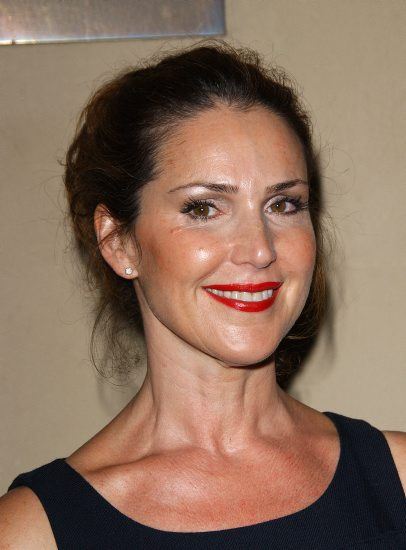
\includegraphics[scale=0.29691]{images/gilpin_female_17.jpg}
    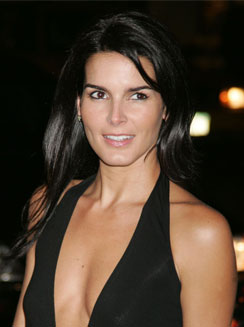
\includegraphics[scale=0.4994]{images/harmon_female_23.jpg}
    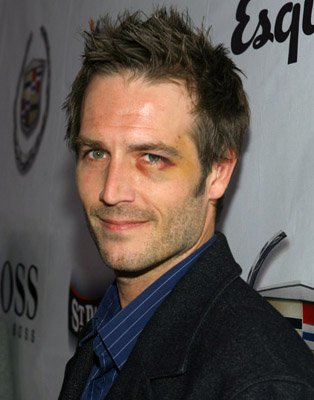
\includegraphics[scale=0.40826]{images/vartan_male_4.jpg}
    \caption{A selection of uncropped photos from the dataset.}
    \label{fig:uncropped}
\end{figure*}

\begin{figure*}[h!]
    \centering
    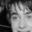
\includegraphics[scale=1.5]{images/radcliffe_male_17.jpg}
    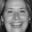
\includegraphics[scale=1.5]{images/bracco_female_138.jpg}
    
\includegraphics[scale=1.5]{images/butler_male_3.jpg}
    
\includegraphics[scale=1.5]{images/merged.png}
    \caption{A selection of cropped, 32x32 grayscale photos from the dataset, the final example is an overlap of examples 2 and 3.}
    \label{fig:cropped}
\end{figure*}

\end{homeworkProblem}
\clearpage
%----------------------------------------------------------------------------------------
%	PROBLEM 2
%----------------------------------------------------------------------------------------

\begin{homeworkProblem}
\noindent \textit{Seperating the dataset}\\
\\
To seperate the data into training, testing, and validation sets, I used a bash script under \texttt{tools/make\_split.sh} which creates 3 new directories (training, testing, and validation) and copies the first 100 images of each actor/actress into the training directory, the next 10 into the testing directory, and the next 10 into the validation directory. Although this is not the best method given that it does not impose any randomness, there are some advantages. Namely, it is clean and simple--which is why I decided to use this method.

\end{homeworkProblem}
\clearpage
%----------------------------------------------------------------------------------------
%	PROBLEM 3
%----------------------------------------------------------------------------------------

\begin{homeworkProblem}
\noindent \textit{Face recognition using k-nearest neighbours}\\
\\
For each image, we find the $k$ nearest neighbours in the training set, and assign to it a prediction which corresponds to the majority of the labels in the set of $k$ nearest neighbours. We define those images which are nearest as the ones with the minimal euclidean distance between flattened grayscale image arrays. $k$ is empirically chosen as $1$, which gives the best performance on the validation set with an accuracy of approximately $78\%$. The performance on the test set for $k=1$ then gives an accuracy of $65\%$.\\
\\
\noindent \textit{Failure cases}\\
\\
\textbf{Error \#1}:
\\
original image: \texttt{vartan\_male\_108.jpg}\\ predicted label: butler\\

Nearest Neighbours:\\
first: \texttt{butler\_male\_2.jpg}\\
second: \texttt{harmon\_female\_32.jpg}\\
third: \texttt{harmon\_female\_71.jpg}\\
fourth: \texttt{butler\_male\_77.jpg}\\
fifth: \texttt{harmon\_female\_18.jpg}\\

\begin{figure*}[h!]
    \centering
    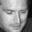
\includegraphics[scale=1.5]{images/vartan_male_108.jpg}\\
    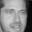
\includegraphics[scale=1.5]{images/butler_male_2.jpg}
    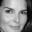
\includegraphics[scale=1.5]{images/harmon_female_32.jpg}
    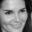
\includegraphics[scale=1.5]{images/harmon_female_71.jpg}
    
\includegraphics[scale=1.5]{images/butler_male_77.jpg}
    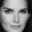
\includegraphics[scale=1.5]{images/harmon_female_18.jpg}
    \caption{The photo on top is the failure case, and the five photos below are the nearest neighbours in order from left to right.}
    \label{fig:e1}
\end{figure*}
\clearpage

\textbf{Error \#2}:
\\
original image: \texttt{radcliffe\_male\_100.jpg}\\ predicted label: vartan\\

Nearest Neighbours:\\
first: \texttt{vartan\_male\_98.jpg}\\
second: \texttt{radcliffe\_male\_67.jpg}\\
third: \texttt{butler\_male\_60.jpg}\\
fourth: \texttt{radcliffe\_male\_16.jpg}\\
fifth: \texttt{radcliffe\_male\_59.jpg}\\

\begin{figure*}[h!]
    \centering
    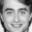
\includegraphics[scale=1.5]{images/radcliffe_male_100.jpg}\\
    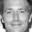
\includegraphics[scale=1.5]{images/vartan_male_98.jpg}
    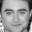
\includegraphics[scale=1.5]{images/radcliffe_male_67.jpg}
    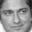
\includegraphics[scale=1.5]{images/butler_male_60.jpg}
    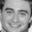
\includegraphics[scale=1.5]{images/radcliffe_male_16.jpg}
    
\includegraphics[scale=1.5]{images/radcliffe_male_59.jpg}
    \caption{The photo on top is the failure case, and the five photos below are the nearest neighbours in order from left to right.}
    \label{fig:e2}
\end{figure*}


\textbf{Error \#3}:
\\
original image: \texttt{gilpin\_female\_105.jpg}\\ predicted label: harmon\\

Nearest Neighbours:\\
first: \texttt{harmon\_female\_40.jpg}\\
second: \texttt{bracco\_female\_64.jpg}\\
third: \texttt{bracco\_female\_34.jpg}\\
fourth: \texttt{gilpin\_female\_23.jpg}\\
fifth: \texttt{gilpin\_female\_17.jpg}\\

\begin{figure*}[h!]
    \centering
    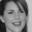
\includegraphics[scale=1.5]{images/gilpin_female_105.jpg}\\
    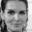
\includegraphics[scale=1.5]{images/harmon_female_40.jpg}
    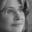
\includegraphics[scale=1.5]{images/bracco_female_64.jpg}
    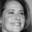
\includegraphics[scale=1.5]{images/bracco_female_34.jpg}
    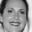
\includegraphics[scale=1.5]{images/gilpin_female_23.jpg}
    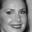
\includegraphics[scale=1.5]{images/gilpin_female_cropped_17.jpg}
    \caption{The photo on top is the failure case, and the five photos below are the nearest neighbours in order from left to right.}
    \label{fig:e3}
\end{figure*}
\clearpage

\textbf{Error \#4}:
\\
original image: \texttt{butler\_male\_106.jpeg}\\ predicted label: radcliffe\\

Nearest Neighbours:\\
first: \texttt{radcliffe\_male\_72.jpg}\\
second: \texttt{butler\_male\_69.jpg}\\
third: \texttt{gilpin\_female\_4.jpg}\\
fourth: \texttt{butler\_male\_40.jpg}\\
fifth: \texttt{radcliffe\_male\_93.jpg}\\

\begin{figure*}[h!]
    \centering
    
\includegraphics[scale=1.5]{images/butler_male_106.jpeg}\\
    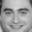
\includegraphics[scale=1.5]{images/radcliffe_male_72.jpg}
    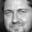
\includegraphics[scale=1.5]{images/butler_male_69.jpg}
    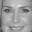
\includegraphics[scale=1.5]{images/gilpin_female_4.jpg}
    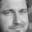
\includegraphics[scale=1.5]{images/butler_male_40.jpg}
    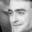
\includegraphics[scale=1.5]{images/radcliffe_male_93.jpg}
    \caption{The photo on top is the failure case, and the five photos below are the nearest neighbours in order from left to right.}
    \label{fig:e4}
\end{figure*}

\textbf{Error \#5}:
\\
original image: \texttt{butler\_male\_102.jpg}\\ predicted label: vartan\\

Nearest Neighbours:\\
first: \texttt{vartan\_male\_63.jpg}\\
second: \texttt{vartan\_male\_96.jpg}\\
third: \texttt{vartan\_male\_59.jpeg}\\
fourth: \texttt{butler\_male\_88.jpg}\\
fifth: \texttt{vartan\_male\_11.jpg}\\

\begin{figure*}[h!]
    \centering
    
\includegraphics[scale=1.5]{images/butler_male_102.jpg}\\
    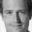
\includegraphics[scale=1.5]{images/vartan_male_63.jpg}
    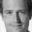
\includegraphics[scale=1.5]{images/vartan_male_96.jpg}
    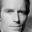
\includegraphics[scale=1.5]{images/vartan_male_59.jpeg}
    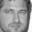
\includegraphics[scale=1.5]{images/butler_male_88.jpg}
    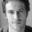
\includegraphics[scale=1.5]{images/vartan_male_11.jpg}
    \caption{The photo on top is the failure case, and the five photos below are the nearest neighbours in order from left to right.}
    \label{fig:e5}
\end{figure*}

\end{homeworkProblem}
\clearpage

%----------------------------------------------------------------------------------------
%	PROBLEM 4
%----------------------------------------------------------------------------------------

\begin{homeworkProblem}
\noindent \textit{Performance results}

\begin{figure*}[h!]
    \centering
    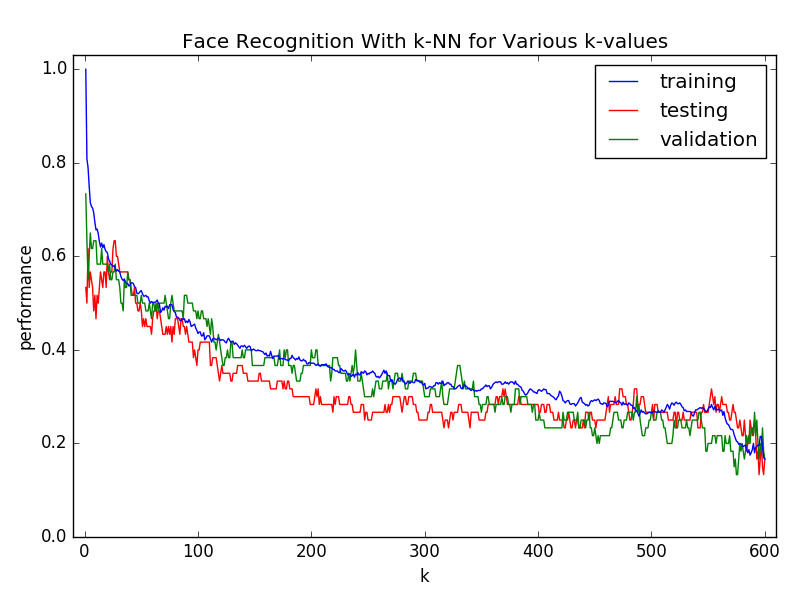
\includegraphics[scale=0.7]{images/graph.png}
    \caption{Performance on training, validation, and testing sets for given values of $k$. Performance is measured as the ratio of correct classifications over total classifications to be made.}
    \label{fig:graph}
\end{figure*}

For very small values of $k$, performance on the training, validation, and testing set is as high as possible. In particular, when $k=1$, performance on the training set is $1$ as expected (the nearest neighbour of an image in the training set is itself). The fact that validation results and testing results are also maximal (or very nearly maximal) at $k=1$ could very well be a coincidence or it could be a result from the structure of the problem. There is no reason why this should happen in general (otherwise we could choose $k=1$ all the time and there would be no need to use a validation set to optimize the $k$ value). Conversely when $k$ is very high, the performance for training, validation, and testing all drop to $1/6$. The reasoning for this is as follows. The majority label of the $k$-nearest neighbours in this case is simply the majority label of the whole training set, which will be a constant for each test case. But since there are an equal number of actors/actresses in the training, validation, and testing sets, precisely $1/6$ of the images will have the predicted label in each data set. This does not necessarily mean that there should be a minimum at $k=600$, though, as there is no reason in principle why the performance can not do worse than random chance. As it turns out, an accuracy of $13\%$ is obtained at $k=599$. In general though, random guessing is a reasonable approximation to the worst case performance, since we are essentially taking random guesses as $k$ becomes very large. Thus, we see that there is a maximum near $k=1$ and a minimum near $k=600$. This explains why the curve tends to decrease as $k$ increases. 

\end{homeworkProblem}
\clearpage

%----------------------------------------------------------------------------------------
%	PROBLEM 5
%----------------------------------------------------------------------------------------

\begin{homeworkProblem}
\noindent \textit{Gender classification using k-nearest neighbours}\\
\\
The method for gender classification is precisely the same as the method described in part 3, except instead of labels for faces we simply use labels which specify whether the person is male or female. The $k$ which gives the best performance on the validation set in this case is $k=1$, with an accuracy of $93\%$. Here is a table which gives the performance for some different $k$-values.\\

\begin{center}
\begin{tabular}{ |c|c| } 
 \hline
 k &  performance\\ 
 1 & 0.93 \\ 
 2 & 0.92 \\ 
 3 & 0.87 \\
 4 & 0.92 \\
 5 & 0.87 \\
 6 & 0.9 \\
 7 & 0.88 \\
 8 & 0.88 \\
 9 & 0.87 \\
 10 & 0.85 \\
 \hline
\end{tabular}
\end{center}

For values of $k > 10$ the performance slowly starts to drop. When the $k$ value of $1$ is used for the testing set, an accuracy of $95\%$ is obtained. The fact that the testing set does better than the validation set in this case is most likely a coincidence, as this should not happen in general (in fact the opposite should happen).

\end{homeworkProblem}
\clearpage

%----------------------------------------------------------------------------------------
%	PROBLEM 6
%----------------------------------------------------------------------------------------

\begin{homeworkProblem}
\noindent \textit{Gender classification with test cases outside of the training set}\\
\\
This is precisely the same procedure described in part 5 except the validation and testing sets contain actors/actresses not included in \textbf{act}. Obtaining this data was done with script \texttt{tools/get\_others.py} (which downloads 10 of each actor/actress for a total of 220 images) and creating the validation and test sets was done with \texttt{tools/make\_other\_split.sh}. The $k$ which gives the best performance on the validation set in this case is $k=4$, with an accuracy of $77\%$. Here is a table which gives the performance for some different $k$-values.\\

\begin{center}
\begin{tabular}{ |c|c| } 
 \hline
 k &  performance\\ 
 1 & 0.65 \\ 
 2 & 0.69 \\ 
 3 & 0.75 \\
 4 & 0.77 \\
 5 & 0.72 \\
 6 & 0.74 \\
 7 & 0.74 \\
 8 & 0.75 \\
 9 & 0.72 \\
 10 & 0.71 \\
 \hline
\end{tabular}
\end{center}

When the $k$ value of $4$ is used for the testing set, an accuracy of $75\%$ is obtained. This performance is $20\%$ worse than the performance obtained in part 5 due to the fact that in part 5, it is very likely that the best approximation to a person's face can be found from another photo of the same person's face, which would likely yield a correct result when classifying gender. In part 6, no such approximation is possible since the person being classified is not part of the training set.

\end{homeworkProblem}
\clearpage

%----------------------------------------------------------------------------------------

\end{document}
